\begin{figure}
\centering
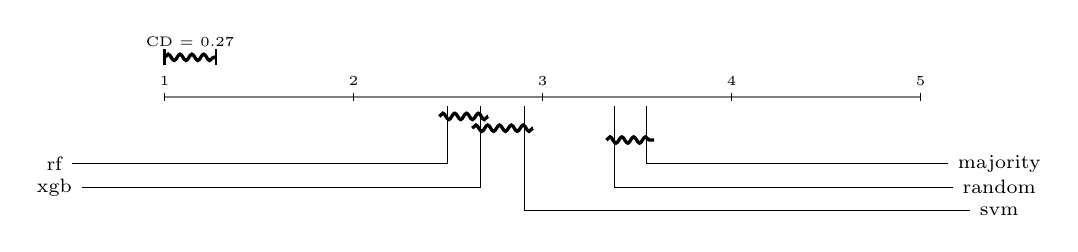
\begin{tikzpicture}[xscale=2]
\node (Label) at (1.362067349834422, 0.7){\tiny{CD = 0.27}}; % the label
\draw[decorate,decoration={snake,amplitude=.4mm,segment length=1.5mm,post length=0mm},very thick, color = black] (1.2,0.5) -- (1.524134699668844,0.5);
\foreach \x in {1.2, 1.524134699668844} \draw[thick,color = black] (\x, 0.4) -- (\x, 0.6);
 
\draw[gray, thick](1.2,0) -- (6.0,0);
\foreach \x in {1.2,2.4,3.6,4.8,6.0} \draw (\x cm,1.5pt) -- (\x cm, -1.5pt);
\node (Label) at (1.2,0.2){\tiny{1}};
\node (Label) at (2.4,0.2){\tiny{2}};
\node (Label) at (3.6,0.2){\tiny{3}};
\node (Label) at (4.8,0.2){\tiny{4}};
\node (Label) at (6.0,0.2){\tiny{5}};
\draw[decorate,decoration={snake,amplitude=.4mm,segment length=1.5mm,post length=0mm},very thick, color = black](2.9441176470588237,-0.25) -- (3.2535294117647053,-0.25);
\draw[decorate,decoration={snake,amplitude=.4mm,segment length=1.5mm,post length=0mm},very thick, color = black](3.1535294117647057,-0.4) -- (3.538235294117647,-0.4);
\draw[decorate,decoration={snake,amplitude=.4mm,segment length=1.5mm,post length=0mm},very thick, color = black](4.005294117647059,-0.55) -- (4.3088235294117645,-0.55);
\node (Point) at (2.9941176470588236, 0){};\node (Label) at (0.5,-0.8500000000000001){\scriptsize{rf}}; \draw (Point) |- (Label);
\node (Point) at (3.2035294117647055, 0){};\node (Label) at (0.5,-1.1500000000000001){\scriptsize{xgb}}; \draw (Point) |- (Label);
\node (Point) at (4.258823529411765, 0){};\node (Label) at (6.5,-0.8500000000000001){\scriptsize{majority}}; \draw (Point) |- (Label);
\node (Point) at (4.055294117647059, 0){};\node (Label) at (6.5,-1.1500000000000001){\scriptsize{random}}; \draw (Point) |- (Label);
\node (Point) at (3.488235294117647, 0){};\node (Label) at (6.5,-1.4500000000000002){\scriptsize{svm}}; \draw (Point) |- (Label);
\end{tikzpicture}
\caption{Nemenyi - input.csv}
\label{fig:nemenyi}
\end{figure}
